\def\year{2016}
\documentclass[letterpaper]{article}

\usepackage{aaai}
\usepackage{relsize}
\usepackage{sectsty}
\usepackage{amsmath}
\usepackage{amssymb}
\usepackage[utf8]{inputenc}
\usepackage[english]{babel}
\usepackage{titlesec}
\usepackage{graphicx} 
\usepackage{wrapfig}
\usepackage{indentfirst}
\usepackage[style=numeric,backend=bibtex]{biblatex}
% For aaai
\usepackage{times}
\usepackage{helvet}
\usepackage{courier}
\setlength{\pdfpagewidth}{8.5in} 
\setlength{\pdfpageheight}{11in}

\setcounter{secnumdepth}{1} % for section number
\addbibresource{reference.bib}

\begin{document}

	\title{Modelling Crimes using Gaussian Processes}
	\author{CS4246 Project Part 1: Gaussian Process (GP) Modeling  \\ \\
	\bf \small Group 5:\\
	\small Choo Boon Yong Martin, A0132760M\\
	\small Leow Yijin, A0131891E\\
	\small Tan Soon Jin, A0112213E\\
	\small Teo Qi Xuan, A0124206W\\
	\small Won Jun Ru Daphne, A0126172M\\
	\small Zhu Liang, A0093910H\\
	}	
	
	\pdfinfo{
		/Title Modelling Crimes using Gaussian Processes
		/Author Martin, Yijin, Soon Jin, Qi Xuan, Daphne, Zhu Liang
	}
	
	\maketitle
	\thispagestyle{empty}
	\pagestyle{empty}
	
	
	%%%%%%%%%%%%%%%%%%%%%%%%%%%%%%%%%%%%%%%%%%%%%%%%%%%%%%%%%%%%%%%%%%%%%%%%%%%%%%%%
	
	\begin{abstract}
	\begin{quote}
		Efficient allocation of police resources is needed to better combat crime. In this paper, we propose to combine the use of heatmaps (kernel-based intensity smoothing) and Gaussian Process (GP) to be explored as a way of modelling crime. By producing a heatmap of risk assessment of crime in a area, it will form an objective guide for law enforcers and planners to better allocate manpower and offer help to the communities.
	\end{quote}
	\end{abstract}
	
	%%%%%%%%%%%%%%%%%%%%%%%%%%%%%%%%%%%%%%%%%%%%%%%%%%%%%%%%%%%%%%%%%%%%%%%%%%%%%%%%
	
	%%%%%%%%%% Section 1
	\section{Introduction}
	
	In this paper, we propose the use of the Gaussian Process (GP) to model the spread of crimes in the District of Columbia (DC).
	The paper will discuss the important requirements of crime models, the way we exploit desirable properties of GP models and the qualitative advantages GP models provide to address the requirements.\\ \\

	The paper will also explain how we train our GP model to predict the crime data, additional insights gained as well as novel modifications of the GP to enhance it. 
	Notably, we touch on how we visualize the output to provide a novel and unprecedented way of interpreting GPs and how the DC authorities can interpret the output.\\ \\

	We then discuss the experimental evaluation of our GP model, particularly how we test it and how the model performs in comparison with other regression models. 
	
	%%%%%%%%%%%%%%%%%% Section 2
	\section{Gaussian Process and Crime}

	In this section, we will briefly describe GPs and our GP model. We then highlight the important requirements of crime modelling, and how our proposed application exploits the desirable properties of GP and its qualitative advantages, as well as how our GP model fits the requirements of crime modelling exactly. 
	Finally, we discuss how the relevant authorities can interpret and exploit the output of the GP model and interact with it.\\ \\

	\subsection{Gaussian Process}
	
	A Gaussian process is a collection of random variables, any finite number of which have a joint Gaussian distribution.
	GP is a non-parametric technique to generalize a set of random variables (r.v.) as a distribution over functions with an infinite dimension. \autocite{c01}
	It is defined by its mean and variance. We define x as a random input variable, $\mu (x)$ as its mean function and $\kappa$ (x, x') as its covariance function resulting in \[f(x) \sim GP(\mu (x), \kappa (x, x')) \]
	Realistically, a GP model is affected by noise, as expressed $y_i = f(x_i) + \epsilon_i$ where $\epsilon_i \sim N(0, \sigma^2_n)$.
	Given observation $\mathbf{y} = [y_1, y_2, \ldots, y_n]^T$, GP will try to infer  $ p(f(\text{x*} | \textbf{y}) \triangleq \mathcal{N}(f(\text{x*}); \mu, \sigma^2)$ where $\mu$ is the prediction and $\sigma^2$ is the predictive variance. 
	
	\subsection{Our Model}
	
	In our GP model, we model all the crimes in a particular district to predict the time and an approximate area at which future crimes are likely to occur.
	We first input various features of past crimes such the Police Service Area (PSA) in charge of the area and the week the crime occurred.
	After processing, we output a heatmap of the likelihood of a specific type of crime occurring in specific areas at specific times, an original and groundbreaking way of visualizing output of GPs.
	
	\subsection{Important Requirements of Crime Models}
	
	Crime occurs continuously and randomly. It is possible for days to go by without any incidents reported, and also possible for multiple incidents to be reported in the same hour.
	Another important factor is that it is possible for a crime to go either undetected or unreported. Thus the model will need to be able to accurately model data with uneven occurrence rates.
	Furthermore, crime can occur as a result of a large number of interdependent factors, most of them unknown and dependent on situation. What drives one criminal to commit crimes may not be the same for another.
	Therefore, the model should not make any assumptions on the features. We should also be able to update the model as more crime occurs, allowing an up-to-date model.\\ \\
	
	\subsection{Desirable Properties of Gaussian Processes}
	
	We thus choose to use GP models to exploit the many advantages it provides in the context of crime.
	The non-parametric nature of GP allows us to model the crime data without making assumptions on the features of crimes.
	The Bayesian property also allows us to update our GP model with information about new crimes as they continue to happen, letting us capture more information about the data as crimes occur.\\ \\

	On the contrary, using a parametric model such as linear regression lacks flexibility to adjust with new datasets, and also requires us to assume features of the crime data.
	It would also be harder to update with new information.\\ \\

	The uneven occurrence rate of crimes creates an uneven sampling rate of sorts.
	Even then, the GP model allows us to use all of the information in the crime dataset to model and predict future crimes.

	The ‘Broken Window’ theory suggests that an area where a crime has occurred is likely to have more crime. \autocite{c07}
	Following this theory, it is highly likely that the crime occurrences in a particular neighbourhood are highly correlated with one another.
	GP model thus provides a good fit for the data.

	\subsection{Output and Interpretation}
	A further advantage of the GP model is that through the predictive mean and uncertainty, we obtain a probability of the crime occurring at a certain area and at a certain time.
	This probability is essential for generating our new and innovative heatmap which will allow the relevant authorities to deploy resources accordingly.
	This is something that regression models such as linear and polynomial regression cannot provide.\\ \\

	Our model outputs a relative risk heatmap for each type of crime, calculated with respect to expected number of crimes, based on the population in a PSA.
	The heatmap is intuitive to interpret, with darker areas being riskier areas.
	It is also possible to output heatmaps of individual crimes if the authorities choose to do so.

	\begin{figure}[!ht]
		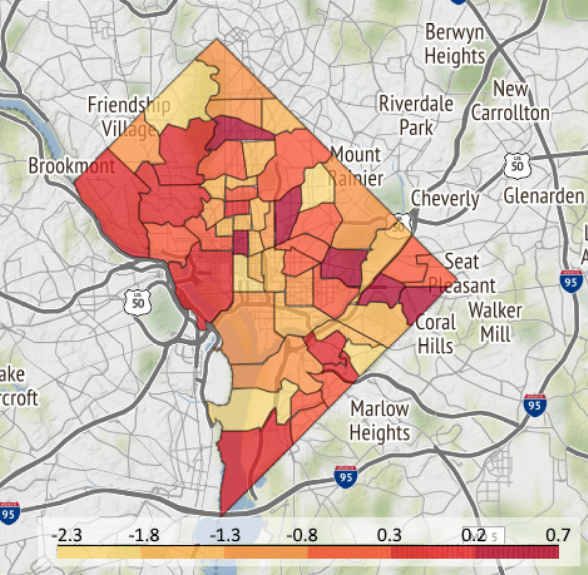
\includegraphics[width=\linewidth]{./p1.png}
		\caption{June 2016 Week 1 Predicted Burglary Log Relative Risk.}
		\label{p1}
	\end{figure}

	This heatmap output can be advantageous in many ways. While we do not know how the DC authorities currently allocates police resources, however it should be reasonable to assume that they would patrol areas with high crime rates previously, i.e. a naive model.
	As such, when we output a heatmap for each type of crime, police officers are able to do pre-emptive tactical planning, based on both the risk level and the types of crimes expected to occur.
	The public can also be informed of the risk of going to those areas. 
	Finally, detecting anomalies from the predicted amount can signal something greater happening, such as gang formation.
	
	%%%%%%%%%%%%%% Section 3
	\section{Technical Approach}
	
	In this section, we will discuss the modelling approach taken for our model, some additional insights gained from this modelling and why our heatmap is really cool.
	
	\subsection{Modelling Approach}
	Using the DC Crime Map dataset, we separated the data by categories. For each category, we aggregated the crime counts by PSA and by week, and train the model on specific categories such as robbery, assault and burglary for the 3-month period of March to May 2016.  For illustration purposes, we will be focusing on the Burglary category.
	As we are dealing with count data that we cannot assume to be mutually independent, unlike the Poisson Process, we model a latent relative risk surface that generates the Cox process (inhomogeneous Poisson Process).
	This is similar to Log Gaussian Cox Process (LGCP) used to model point process.
	To predict the likelihood of a crime, we use a poisson distribution. Due to its non-Gaussian characteristic, we approximate an inference with Laplace Approximation by utilizing the second order Taylor series, or the following formula:
	\[p(y|f) = \prod_{s,t}Poisson(y_{s,t}|exp(f(s,t))\cdot e_s)\]

	This likelihood function was chosen as count data must be positive real values, hence Gaussian likelihood was bound to fail.
	In selecting the kernel, we we followed recommended kernels from paper which combined multiple kernels to investigate the effect of different input dimensions:
	\[K((s,t),(s',t')) = k_s(s,s')+k_t(t,t')+k_{st}((s,t),(s',t'))\]

	We experimented with the different kernels and compared their results.
	\begin{table}[!ht]
		\begin{tabular}{| p{2.5cm} | l | p{2cm} | p{2cm} | }
		\hline
		Kernel & Robbery & Burglary \\ \hline
		Space & 136.3020284 & 61.07216753\\
		Time & 3.430992165 & 1.215659926\\
		Space-Time & 24.68697493 & 2.832692267\\
		Periodic & 44.83034608 & 21.92304832\\
		Combined & 25.93114219 & 3.144605593\\
		\hline
		\end{tabular}
		\caption{Comparisons of kernels}
		\label{t1}
	\end{table}
	In the combined version, we use the Matern ${3}\over2$ kernel for space, Radial Basis Function kernel for time, as well as the periodic Matern 3/2 kernel.
	We then maximize the marginal likelihood by optimizing using Limited-Memory Broyden–Fletcher–Goldfarb–Shanno (LBFGS).
	We chose the LBFGS method as it gave the best result of all the methods tried, including Scaled Conjugate Gradients and Truncated Newton method.
	
	We chose to model specific crimes separately, after learning the hard way when we attempted to predict on the combined crime counts. We were also able to integrate widely available spatiotemporal data online to perform forecasting which achieved good results with only 3 months of training data.
	
	\subsection{Additional Insight}
	Through the undertaking of this project, we have derived several additional insights about the GP model:
	\begin{enumerate}
		\item {\bf Pattern Discovery:} We can use a more expressive kernel from a learned covariance function to learn hidden representations of data. \autocite{c03}
		\item {\bf Feature Selection:} It is possible to use ARD (Automatic Relevance Determination) covariance function to perform feature selection on different inputs for a crime problem. \autocite{c04}
		\item {\bf Log-Cox Gaussian Process:} It is possible to apply LGCP to investigate the contagious effect of crime. \autocite{c05}
		\item {\bf Stationarity of data:} We experimented with non-stationary kernel, assuming the data was stationary.
		\item {\bf Mean Function:} We learned the importance of setting mean function properly to indicate bias.
		\item {\bf Incorporation of Side Data:} Another advantage of the GP is the possibility of incorporating side information by coupling together multiple Probabilistic Matrix Factorization problems. \autocite{c02}
	\end{enumerate}
	
	\subsection{Novel and Interesting Heatmap}
		As discussed in the earlier Output and Interpretation section, our group has thus focused on the visualization of the GP model output in order to exploit the many advantages of GP and the intrinsic user-friendliness of heatmaps.
	In doing so, we have created a novel heatmap GP visualization that will enable the relevant authorities to better make an informed decision on how to best allocate police resources.
	
	%%%%%%%%%%%%%%%% Section 4
	\section{Experimental Evaluation}
	The usefulness of a GP model depends on many factors. As such, there is a need to empirically evaluate its performance.
	In particular, we focus on how our model will be used to enable efficient allocation of police resources to combat crime.

	\subsection{Testing of GP}
	For efficient allocation of police resources to combat crime, we place an emphasis on accuracy of crime predicted and ease of interpreting output. 
	We use accuracy to compare with other models. To measure accuracy, we use mean square error (MSE) to benchmark our model against the state-of-the-art alternatives \autocite{c06}. During the test, we arbitrarily chose to use the Combined kernel in our model for experimentation.

	\subsection{Comparison with Current Methods}
	
	To get an indication of how useful our model is, we then perform the same test on out-of-sample data.
	We thus compare our model against both the state of the art model and a naive forecast model with Holt-Winters smoothing.
	
	\begin{figure}[!ht]
		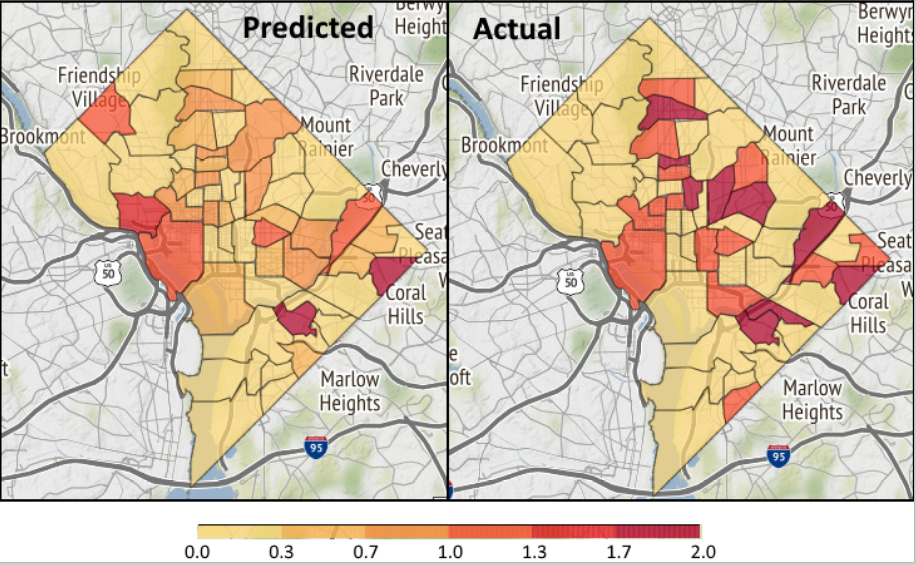
\includegraphics[width=\linewidth]{./p2.png}
		\caption{Predicted and Actual Robbery Crimes in June 2016 Week 1.}
		\label{p2}
	\end{figure}

	\begin{table}[!ht]
		\begin{tabular}{| p{1cm} | l | p{2cm} | p{1.5cm} | }
		\hline
		& Our Model & State-of-the-Art Model & Holt-Winters \\ \hline
		Out-Sample Error & 3.144605593 & 5.080 & 6.855\\
		\hline
		\end{tabular}
		\caption{MSE of our model against state-of-the-art models and naive with Holt-Winters.}
		\label{t2}
	\end{table}

	As can be observed from the MSE values, our model does better than the state-of-the art model as well as Holt-Winters method in predicting the Burglary crimes, which we were pleasantly surprised about. However, when used on other categories of data, such as Robbery, the MSE does not perform as well, probably due to unsuitable use of the kernels in the robbery context.
	
	%%%%%%%%%% Section 5
	\section{Evaluation}
	Our model also outputs multiple forms of heatmaps. Each heatmap can be used by the police for different purposes, but in general, the motivation for producing them is so that the police will be able to better manage their resources (which are expensive and limited), to make it a safer place for citizens to live in.
	\subsection{Relative Risk}
	\begin{figure}[!ht]
		\minipage{0.15\textwidth}
		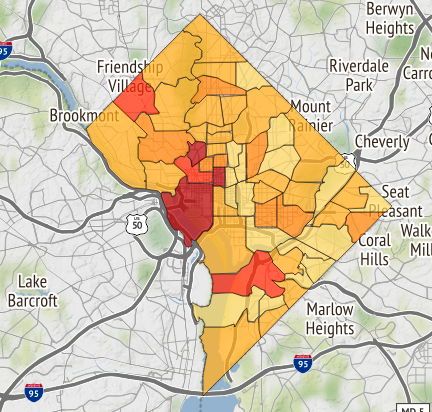
\includegraphics[width=\linewidth]{./w22_relative.png}
		\caption{Relative risk of crimes in Week 22}
		\label{p3}
		\endminipage\hfill
		\minipage{0.15\textwidth}
		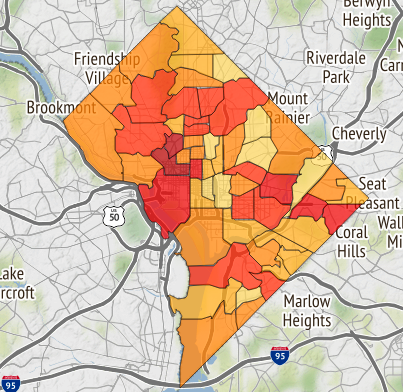
\includegraphics[width=\linewidth]{./w23_relative.png}
		\caption{Relative risk of crimes in Week 23}
		\label{p4}
		\endminipage\hfill
		\minipage{0.15\textwidth}
		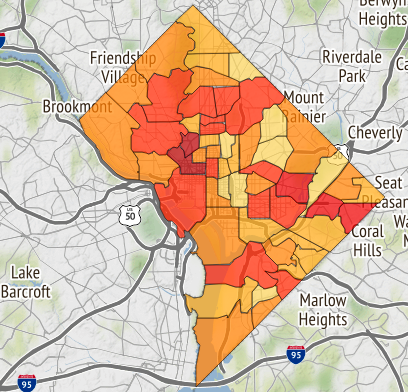
\includegraphics[width=\linewidth]{./w24_relative.png}
		\caption{Relative risk of crimes in Week 24}
		\label{p5}
		\endminipage\hfill
	\end{figure}
	The main output of our model is the relative risk heatmap. This heatmap is adjusted to the expected count of crimes in the area, based on the population, instead of being based on the absolute amount. If the predicted count is far above the expected count for the area, they are considered to be of higher risk, and will be darker as shown in the figures. This visual information will easily allow the police to identify which areas are likely to require more police resources, including people, and make preparations for it. Putting the heatmaps for each week side-by-side will also allow the police to better understand the spread of crimes across the areas, and possibly identify underlying causes for the phenomenon.
	\subsection{Anomaly Detection}
	\begin{figure}[!ht]
		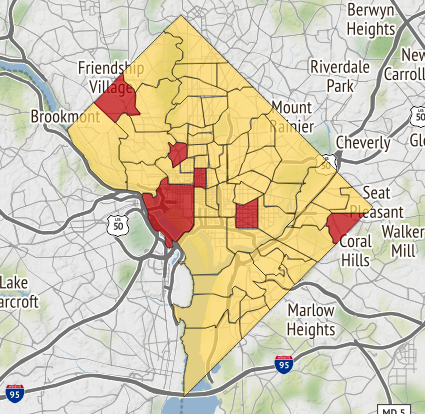
\includegraphics[width=\linewidth]{./w22_outlier.png}
		\caption{Mapping of Anomalies}
		\label{p4}
	\end{figure}
	Another output that our model produces is the anomaly map. Using this map, the police are able to identify which areas have unexpected amount of crimes, whether it be too high or too low. Using this information, the police can initiate a thorough investigation into the cause. For example, the increased amount of crimes could be due to emergence of crime syndicates in the region. If the police are able to investigate and uncover this, they can tackle the problem in the bigger picture of tracking down these crime syndicates, rather than simply attempting to arrest the burglars. This is a way that the police can make better use of their resources.

	\subsection{Variance analysis}
	\begin{figure}[!ht]
		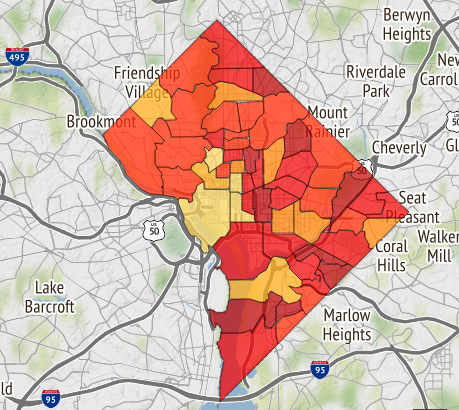
\includegraphics[width=\linewidth]{./w22_variance.png}
		\caption{Variance map}
		\label{p5}
	\end{figure}
	Last, but not least, our model is also able to output a variance heatmap. Having too high of a variance suggests that the model is not confident of its prediction in that area. This could instigate the police to increase the amount of patrol in these areas, so as to be able to spot crimes that may go unreported. This will also improve the future predictions of the crimes in the area since more data will be available for the model.
	
	%%%%%%%%%% Section 6
	\section{Conclusion}
	In this paper, we have proposed an innovative way of combining the rich class of Gaussian Processes and the visually interpretable heatmap to create an easily interpretable risk assessment of crime in a area.
	Although our model slightly underperforms when compared with the latest state-of-the-art model, we believe that the slight dip in accuracy is an acceptable trade-off for the more user-friendly output.
	It is also likely that enhancing our model with side information that the authorities have access to will enable us to outperform the state-of-the-art model.
	
	%%%%%%%%% Section 7
	\section{Members}
	\begin{itemize}
		\item {\bf Choo Boon Yong Martin (A0132760M), Leow Yijin (A0131891E) and Tan Soon Jin (A0112213E)} were in charge of modelling the data.
		\item {\bf Teo Qi Xuan (A0124206W) and Won Jun Ru Daphne (A0126172M)} were in charge of writing the report.
		\item {\bf Zhu Liang (A0093910H)} was in charge of processing the data and visualization.
	\end{itemize}

	%%%%%%%%%% References

	\printbibliography

\end{document}